\scanpage{19}
% Foliotation archivistique au crayon, en bas à gauche : 18.
\diagram{\begin{tikzcd}[ampersand replacement=\&,column sep=large,row sep=large]
X'=\mathbb P^1_{\mathbb Q} \arrow[r,no head] \arrow[d,"{\mu_{n\,\mathbb Q}}"'] \& \bar X' \arrow[d,no head] \\
X=\mathbb P^1_{\mathbb Q} \arrow[r,no head] \arrow[d,no head] \& \bar X \arrow[d,no head] \& 0,1,\infty,-j,-\bar j \\
\mathbb Q \arrow[r,no head,"\Gamma"'] \& \overline{\mathbb Q}
\end{tikzcd}}
\[f(z)=z^n\]
\diagram{\begin{tikzcd}[ampersand replacement=\&,column sep=large]
1 \arrow[r] \& \mu_n(\overline{\mathbb Q}) \arrow[r] \& \mathcal E_n \arrow[r] \& \Gamma \arrow[l,bend left=25] \arrow[r] \& 1
\end{tikzcd}}
\[\mathcal E_n=\Gamma\cdot\mu_n(\overline{\mathbb Q})\]
\[
\left\{\begin{aligned}
&S_0=\{0\},\quad S_1=\mu_n(\overline{\mathbb Q}),\quad S_\infty=\{\infty\}\,,\\
&E^+=\{z\mid z^n=-j\}\\
&E^-=\{z\mid z^n=-\bar j\}
\end{aligned}\right.
\]
\deleted{$f(z)$}
\[
E=\{z\mid z^{3n}=-1\deleted{\}},\ z^n\ne-1\}
\]
\[
\begin{aligned}
R'&=\{z\mid z^n=\tfrac12\}\\
R''&=\{z\mid z^n=2\}\\
R&=\{z\mid z^n=-1\}
\end{aligned}
\]
\margin{$R$}
\[E\cup R=\{z\mid z^{3n}=-1\}\]
\[
\begin{array}{c}
\mathbb Q[E\cup R]=\mathbb Q[\mu_{6n}(\overline{\mathbb Q})]\\
\bigcup\\
\mathbb Q[S_0\cup S_1\cup S_\infty]
\end{array}
\]
\[
\mathbb Q[R',R'']\deleted{\unsure{R}}=\mathbb Q[R']=\mathbb Q[\sqrt[n]{2}]
\]
\figure{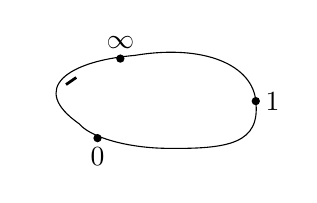
\begin{tikzpicture}[x=1cm,y=1cm]
\draw (0,0) .. controls (-.65,.45) and (-.15,.8) .. (.7,.87)
 .. controls (1.6,1.02) and (2.2,.74) .. (2.24,.29)
 .. controls (2.3,-.25) and (1.9,-.32) .. (1.1,-.31)
 .. controls (.55,-.3) and (.12,-.15) .. (0,0);
\draw[line width=1pt] (-.17,.5) -- (-.04,.59);
\fill (.52,.83) circle (1.5pt) node[above] {$\infty$};
\fill (2.24,.29) circle (1.5pt) node[right] {$1$};
\fill (.23,-.18) circle (1.5pt) node[below] {$0$};
\end{tikzpicture}}
\diagram{\begin{tikzcd}[ampersand replacement=\&,column sep=large]
1 \arrow[r] \& \mu_\nu(\overline{\mathbb Q}) \arrow[r] \& \Gamma'_{\deleted{\unsure{n}}} \arrow[r] \& (\mathbb Z/n\mathbb Z)^* \arrow[r] \& 1
\end{tikzcd}}
$\nu=\text{ordre de }2\text{ dans }\deleted{\unsure{\mathbb Q^*}}\ K_n^*/K_n^{*n}$, où $K_n=\mathbb Q(\sqrt[n]{1})$.
\[
\begin{array}{rcll}
0,1,\infty&\longmapsto&0&\text{ordre }2\\
\tfrac12,2,-1&\longmapsto&1&\text{ordre }2\\
-j,-\bar j&\longmapsto&\infty&\text{ordre }3
\end{array}
\]
\par\noindent\rule{.7\linewidth}{.2pt}
\[
g(z)=\frac{27z^2(z-1)^2}{4(z^2-z+1)^3}\qquad
 gf(z)=\frac{27}{4}\frac{z^{2n}(z^n-1)^2}{(z^{2n}-z^n+1)^3}
\]
\[\lambda\frac4{27}=1\]
\[
g(z)=1\Longleftrightarrow
\underbrace{4(z^2-z+1)^3-27z^2(z-1)^2}_{\begin{aligned}
&\unsure{-4|4}\bigl[(z+1)(z-\tfrac12)(z-2)\bigr]^2
=4\bigl[(z+1)(z^2-\tfrac52+1)\bigr]^2\\
&\hspace{6em}=\bigl[(z+1)(2z^2-5+2)\bigr]^2
\end{aligned}}=0
\]
% Dans les deux derniers facteurs, aucun z distinct n'est visible après 5/2 ni après 5 ; aucune correction algébrique n'est introduite.
